\newpage
\chapter{Results}
\label{experiment_results}
\lhead{\emph{Experimental Results}}
We first present a full replication and extension of the work by
\citet{radDeliberationSinglePeakednessCoherent2021}. Then we present the simulations based on our model of
meta-deliberation, as well as the results of the sensitivity analysis on both
models. All code for the replication, main experiment and visualizations can be
found in \href{https://github.com/amirsahrani/master_thesis}{this Repository}. \Cref{AppendixB} contains all the values and ranges used for the experiments, as well as supplementary figures.


\section{Replication}\label{sec: replication} We are able to fully replicate the results found by
\citet{radDeliberationSinglePeakednessCoherent2021},  in \Cref{fig:rep_cyclic}
we see that for the biases less than 0.73, all metric results in acyclic
preferences. We also replicate the behavior of the KS metric, where biases in
the range of 0.73-0.85, show that even initially acyclic profiles can become
cyclic. \Cref{fig:rep_count} Further explains this by showing that within this
range we always observe 3 unique profile for the KS metric, while DP and CS
have already settled on 6 profiles, thereby representing all possible
preferences. \Cref{fig:rep_condorcet} shows KS introduces ambiguity in the case
that there was a Condorcet winner, resulting in losing the original nice
profile. Finally, the proximity to single-peakedness shows a slightly more
positive note for the KS metric, showing that while the DP and CS bottom out to
the minimum proximity to single-peakedness, KS stays relatively close. Though
this should be taken with a grain of salt, as it is likely a consequence of the
unique preferences being smaller.

\begin{figure}[htbp]
	\centering
	\begin{minipage}{0.45\textwidth}
		\centering
		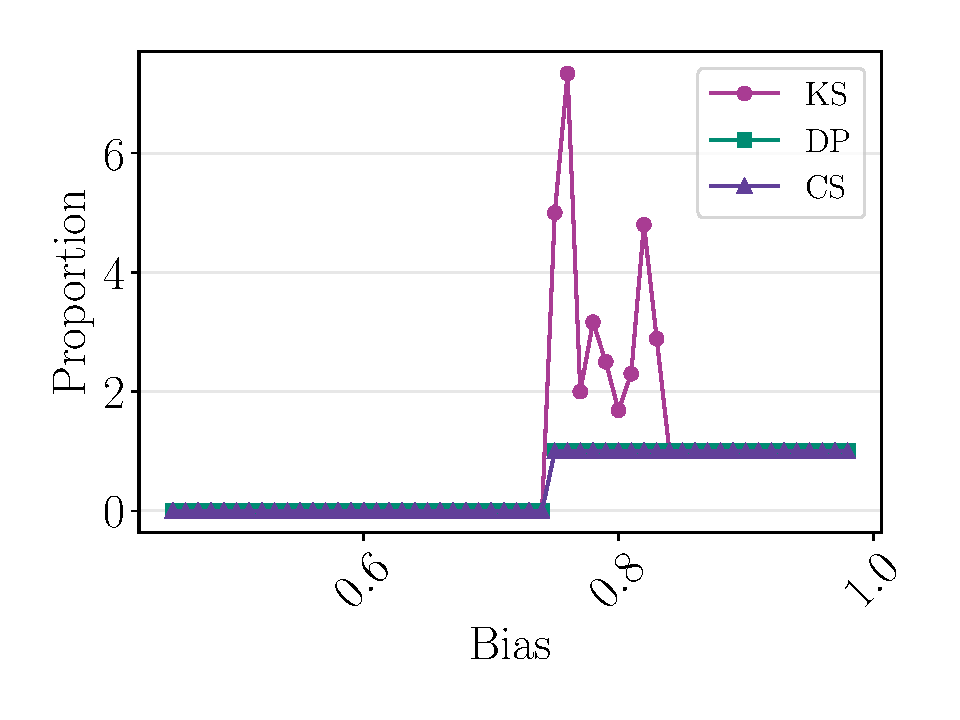
\includegraphics[width=\textwidth]{Figures/cyclic_proportion_Proportion.pdf}
		\caption{The proportion of cyclic profiles remaining, 0 indicating that no cyclic profiles were present after deliberation.}
		\label{fig:rep_cyclic}
	\end{minipage}\hfill
	\begin{minipage}{0.45\textwidth}
		\centering
		\vspace{-9pt}
		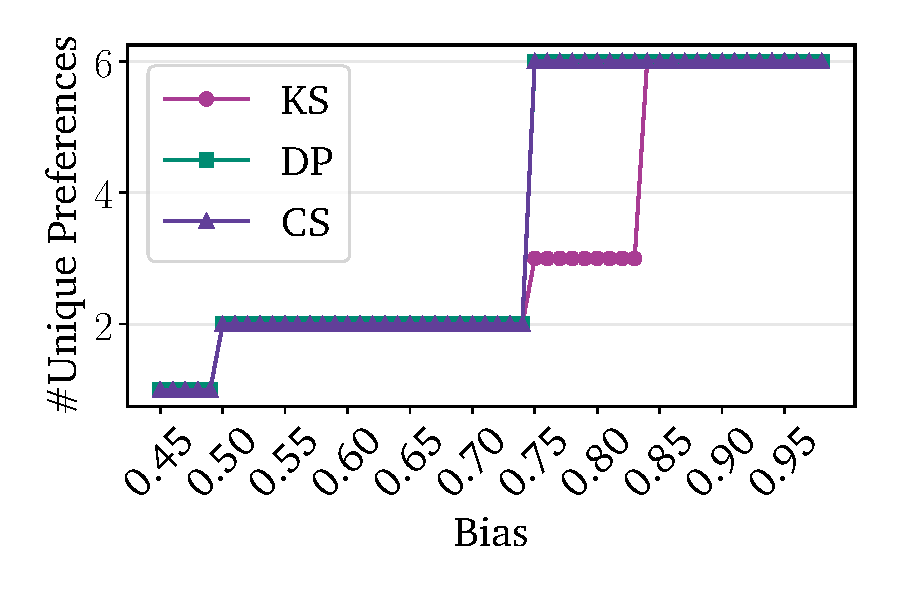
\includegraphics[width=\textwidth]{Figures/unique_Unique Preferences.pdf}
		\caption{Number of unique preferences at the final step of deliberation.}
		\label{fig:rep_count}
	\end{minipage}

	\vspace{1em}

	\begin{minipage}{0.45\textwidth}
		\centering
		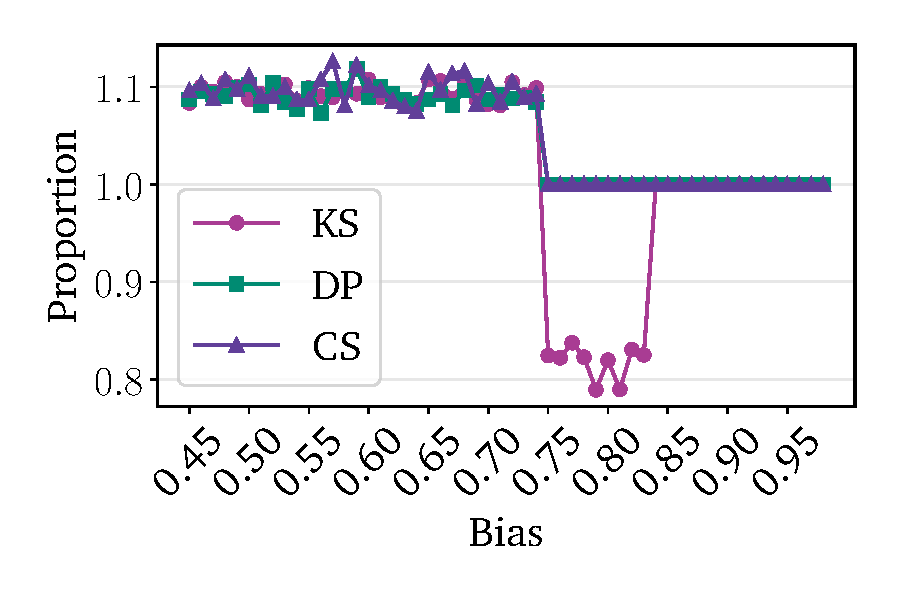
\includegraphics[width=\textwidth]{Figures/condorcet_proportion_Proportion.pdf}
		\caption{The proportion of Condorcet winners left after deliberation, value above one indicate Condorcet winners emerging during deliberation}
		\label{fig:rep_condorcet}
	\end{minipage}\hfill
	\begin{minipage}{0.45\textwidth}
		\centering
		\vspace{-9pt}
		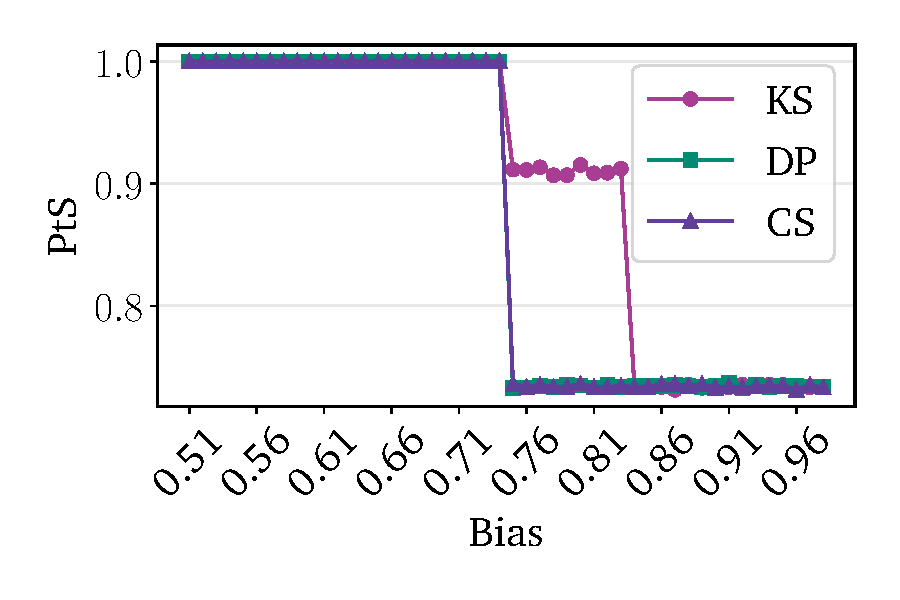
\includegraphics[width=\textwidth]{Figures/sp_proximity_PtS.pdf}
		\caption{Proximity to single-peakedness after deliberation. Proximity to single-peakedness as defined in \Cref{section:related_work}.}
		\label{fig:rep_single_peaked}
	\end{minipage}
\end{figure}



% https://onlinelibrary.wiley.com/doi/10.1002/bimj.202200091
% Things that might end up going into the methods section, but need to be mentioned:
% [X] How is any source of randomness generated
%	If Original groups are used, the only source of randomness is the group that we choose to measure and the voter(s) used to generate the potential candidates
%	If we do not use original groups, then we randomly select voters (uniformly at random)
%	[X] In each case the uncertainty over the candidates is modelled as a normal distribution with mean 0 and std 2
% How are the parameters sampled
%	For sensitivity: Sobol (Side note explain sensitivity analysis)
%	For other experiments: Simply uniform sampling
%	Sample size: Sensitivity chosen such that there are no negative indices, acknowledge that this might result in smaller error bars. Other: We pick 1000, though power analysis would likely be better, limited in number of samples because of the NP-hardness of PtS-V
% [X] What are we trying to estimate
%	We are trying to estimate the final PBS
%	For this we want the smallest average distance between final PBS and simulated PBS
% How are we measuring the performance of the model
%	Absolute difference, since the errors are small there absolute difference and the squared difference are similar.
% How are we going to test this performance
%	We simply look for the best this model can do, and given that we try to explain what factors are important when considering an explanatory model of deliberation.


% Things I need to do: 
% Explain general experimental setup, small recap of what
% we are going to present. Restate the goal of the analysis. How we adapted the
% original data to fit our study, mainly only using voters that have filled in
% both pre and post questionnaires without missing data. Report the number of
% voters before and after this clean up. 

% [X] Show relplots of knowledge and pbs.


\newpage
\section{DeGroot Model}\label{degroot_results}

% Intro
We present the results based on the DeGroot model. The model is informed by the
data from the \textsc{America in one Room} experiment, which was used to
construct the support vectors $\Support$ as well as the estimated support
matrices $\EstSupport$. We follow the original paper, focussing on the most
polarizing questions,  as mentioned in \Cref{sub:americainonroom}, the
policy-based ideology score (PBS) is the average of the 26 most polarizing
questions, where a low PBS corresponds to more liberal answers, and high PBS
indicates more conservative answers.

% Data usage
We remove all participants with missing responses to any pre- or
post-deliberation measurements, retaining only voters with complete pre- and
post-deliberation data. As a result, only 247 out of the original 523 opinions
remain after this selection. Though this removes a large fraction of voters,
given that this model makes quite strong assumptions on voting behavior for
which we do not have data, we limit our testing to voters of which we can be
sure that we know their true opinion. The support vectors $\Support$ correspond
to the voters' reported opinions, based on measured by several policy questions
rated from 0 to 10 (inclusive). Each voter's estimated support matrix
$\EstSupport$ is generated by adding normally distributed noise($\mu=0$, $\sigma=1.37$) to the
candidates' true opinions. The mean of 0 ensures we do not bias the model towards
preferring candidates with higher or lower average scores, as otherwise people
would consistently be over or underestimating candidates' support. The standard
deviation is chosen to match voter PBS distribution before
deliberation.
% Discussion: The normal distribution might not be realistic at all. The
% distribution can be skewed, and the means can be different from 0. Also
% likely different for different demographics


% Simulation parameters
To generate a deliberation groups, we opt for two approaches. Either using the
original deliberation groups, selecting a group at random and using the voters
from that group. Given the restriction of voters with complete data these
groups will tend to be smaller than in the original study, where these groups
averaged 13 voters, in our subsection the average is 7. Or we generate new
groups by picking $n$ voters uniformly at random without replacement and
placing them into a single group. Disregarding any similarity to the original
structure the groups might have had.

% Simulation performance
To evaluate model performance, we predict each voter's post-deliberation
opinion and compare it to the observed data. Additionally, we group voters into
$m$ bins based on their initial PBS and compare the average predicted opinion
within each group to the actual group average. This effectively model
substantive agreement and thus does not incorporate \textit{meta-agreement}.
However, it allows for the evaluation of the model without assumptions on how
to infer the final ``preferences'' of the voters, or the opinions of
candidates. After this assessment, we investigate the convergence of the model,
as well as its sensitivity to the choice of parameters.

% We now assume that substantive agreement and meta-agreement happen at the same pace, but in practice this might be unrealistic as people talk about one topic at a time, and there might be complex dynamics between them. For example learning that you have strongly misjudged a candidate might result in you sticking to your substantive opinion

% Extension to meta agreement
Finally, we extend the model to incorporate meta-agreement through deliberation on the trust matrices. Assessing its effect on voters’ final preferences, using the metrics introduced in \Cref{sec: replication}.

\subsection{Policy-Based Ideology Scores}

We first proceed with analyzing the performance of the DeGroot model with
respect to substantive agreement. \Cref{fig:pbs} shows the PBS of both the
deliberation and control group, and the simulation results for both instances.
As expected the model performs poorly at predicting the control group, as there
was no significant change for control group members in the original data.
Within the deliberation group, a voter's initial PBS remains a strong indicator
of their final PBS. We observe that the models predictions get more accurate
after the first time step, with prediction errors increasing over time. This is
because the model causes voters to converge too strongly, thereby eliminating
most extreme opinions, contrary to the real data. The implications of this
depend on the nature of long term deliberation. If, as suggested by
\citet{elsterMarketForumThree2002}, deliberation is able to reach full
consensus, the model might offer a plausible approximation of this process.
However, if full consensus is not typically reached—as is precisely the
motivation for incorporating meta-agreement into the model—then the DeGroot
model should be seen as overly simplistic in its assumption that individuals
converge toward a weighted average of the opinions presented to them.

\begin{figure}[ht]
	\begin{center}
		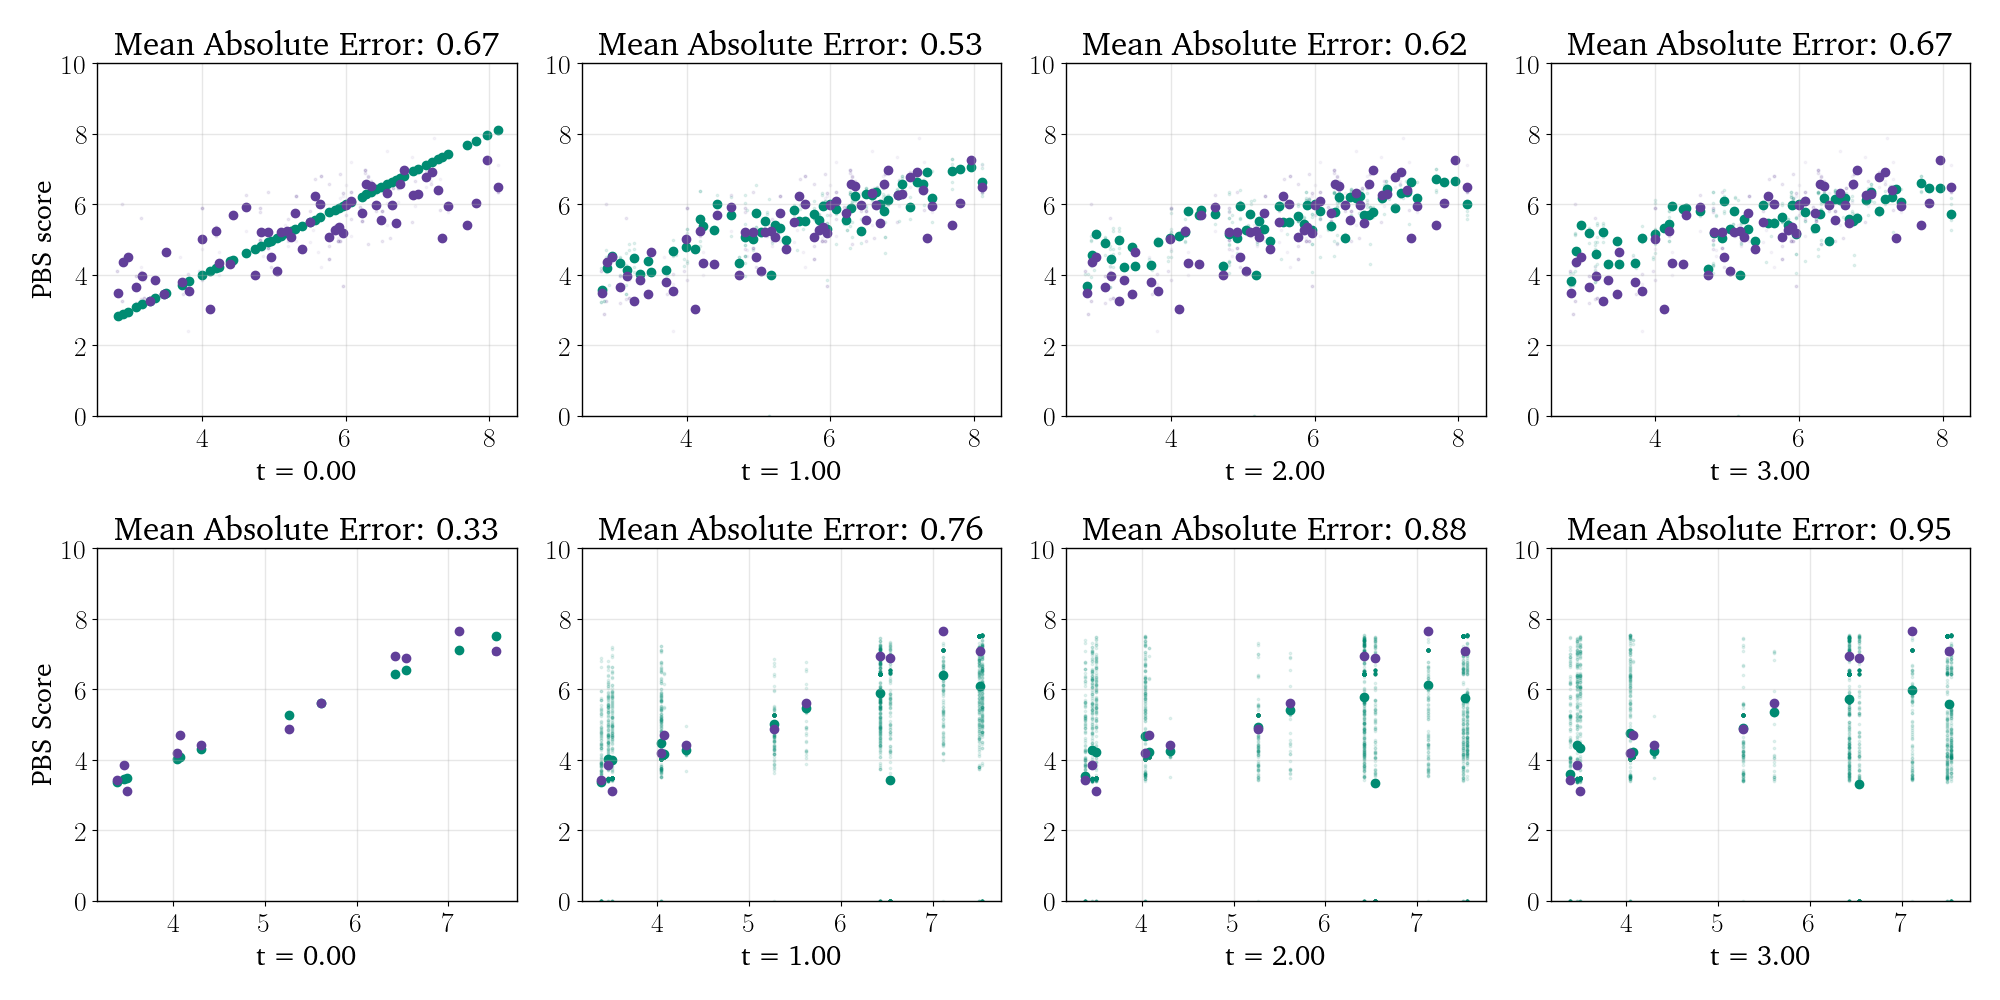
\includegraphics[width=0.95\textwidth]{Figures/pbs_scores.png}
	\end{center}
	\caption{ PBS, purple indicating the PBS after deliberation in the original data, green indicates the results of the simulation in that time step. Large dots indicate the binned data, smaller dots indicate individual voters.}\label{fig:pbs}
\end{figure}

\Cref{fig:delta_pbs} depicts the change in PBS within the deliberation
group. In the original data, we see that most changes occur among participants
with high initial PBS, who tend to moderate their views. The model, by
contrast, predicts the most significant changes among those with low PBS in
later time steps.

One possible explanation for this discrepancy is the correlation between PBS
and political knowledge. As shown by \citet{fishkinCanDeliberationHave2024},
voters with more extreme PBS also tend to be more knowledgeable. Our
filtered dataset supports this, showing a weak negative correlation of -0.05
($p < 0.5$), \Cref{fig:knowledge_pbs} in~\Cref{AppendixB}
shows the distribution of political knowledge across different PBS ranges.
Since political knowledge in our sample is skewed toward voters with high PBS,
incorporating knowledge-based trust into the model amplifies their influence,
resulting in larger prediction errors.

However, \Cref{fig:binned_errors} shows that the model performs better when
knowledge is excluded from the trust calculation. This suggests that political
knowledge, at least as measured in this dataset, is a poor predictor of
persuasiveness. It should be recalled, that the knowledge questions assess factual
knowledge of the U.S. government, such as knowing which party holds a
Senate majority, which may not correlate well with persuasiveness on substantive
issues such as immigration or economics.


\begin{figure}[ht]
	\begin{center}
		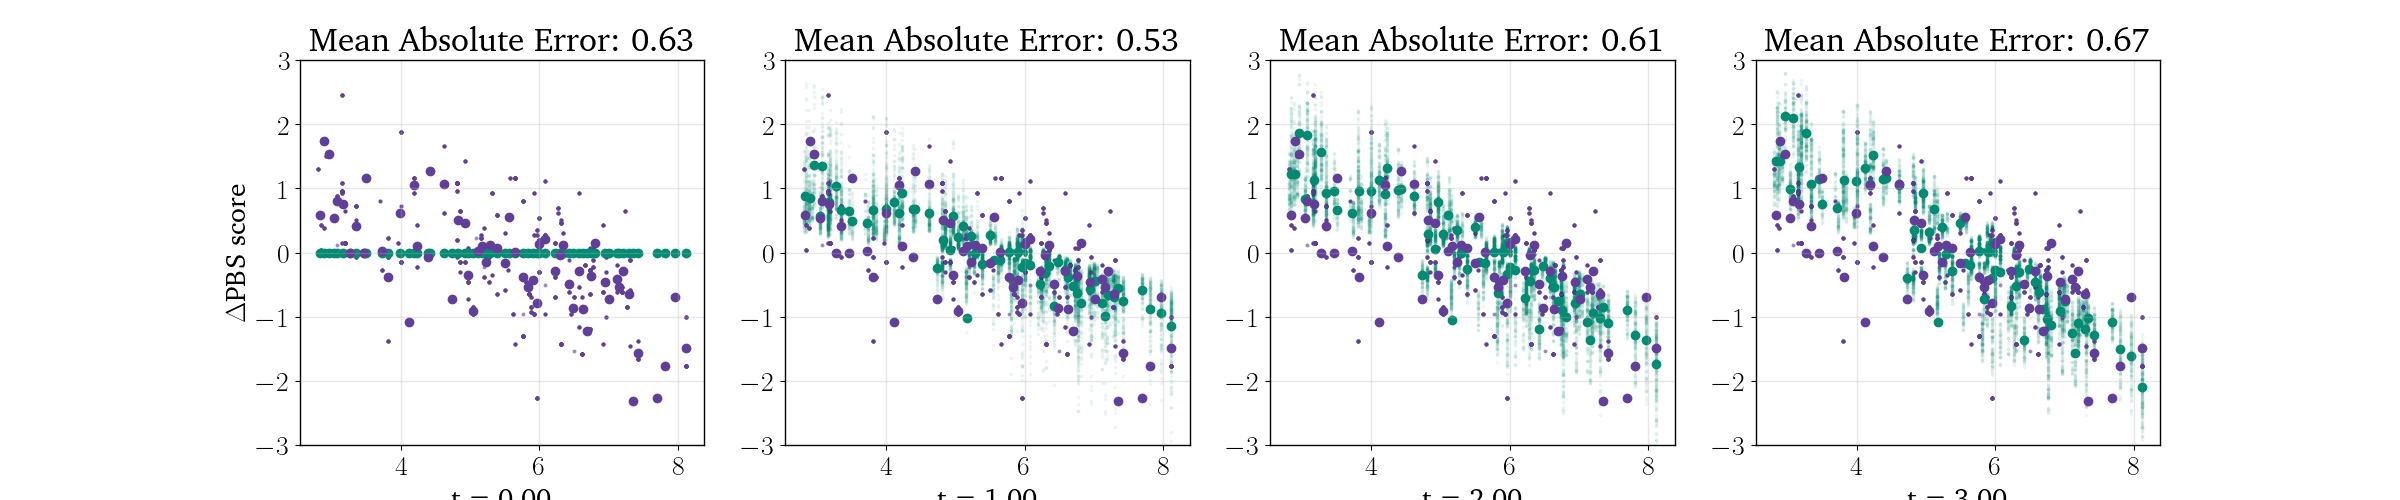
\includegraphics[width=\textwidth]{Figures/change_pbs_scores.png}
	\end{center}
	\caption{Change in  PBS, relative to the original, pre deliberation, measurement. The control is  omitted as there was no significant change.}\label{fig:delta_pbs}
\end{figure}


We note that these slightly positive results appear only when the voters are
grouped by their original PBS, thereby giving the model reasonable predictive
power over a population of voters.  This holds even for different number of
bins. \Cref{fig:binned_errors} shows the progression of errors over time when
the error is calculated on a per-individual basis, and we find the model
consistently overestimates the change in PBS, and thereby gives a worse
prediction than the initial PBS.

\begin{figure}[ht]
	\begin{center}
		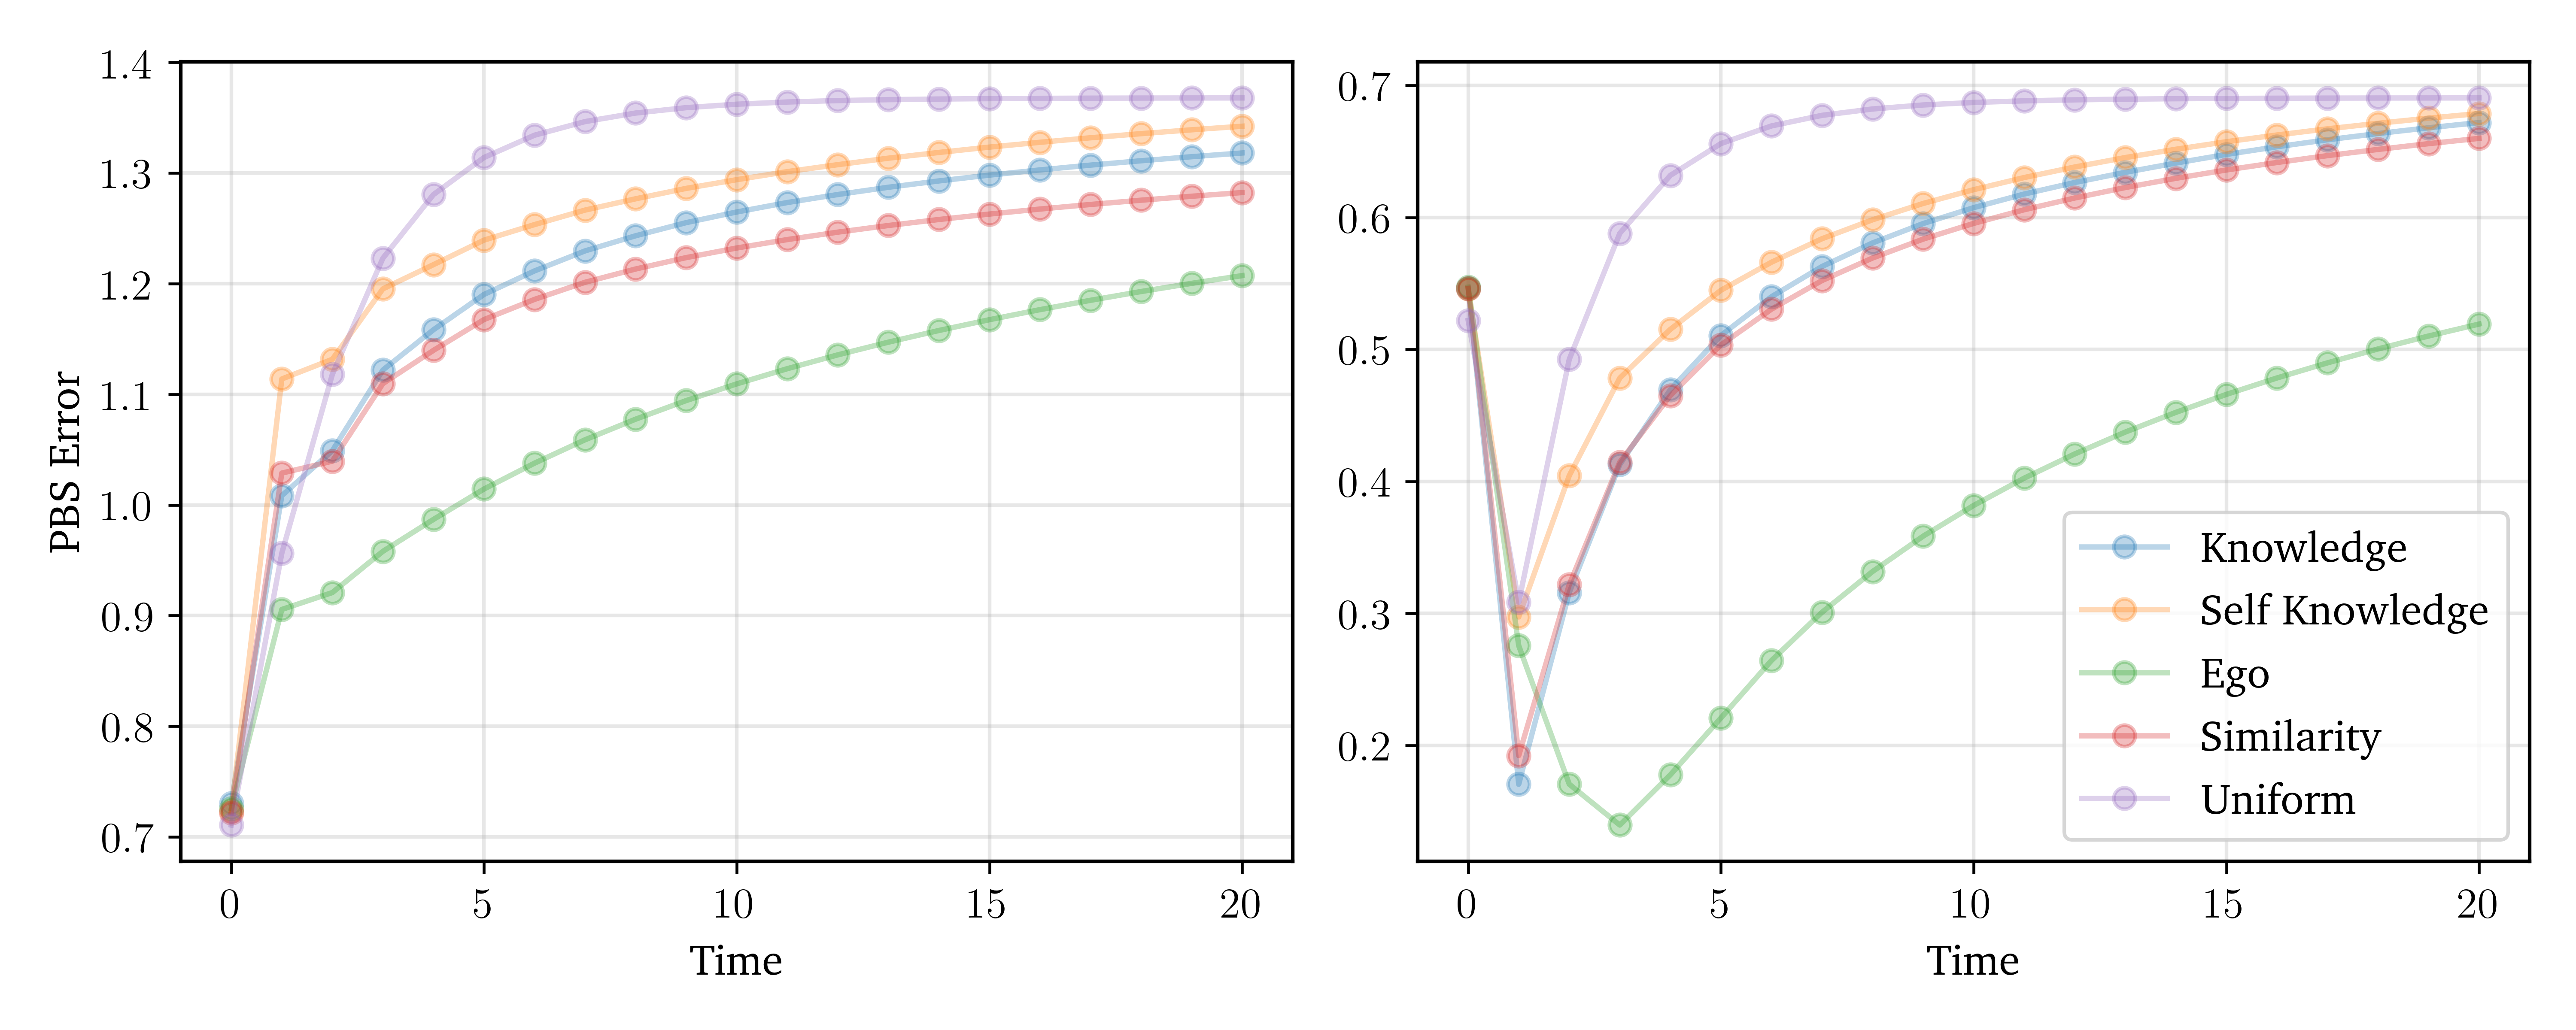
\includegraphics[width=0.95\textwidth]{Figures/errors_binned.png}
	\end{center}
	\caption{Prediction error of the model as a function of time, binned relative to the original  PBS.}\label{fig:binned_errors}
\end{figure}


\begin{figure}[ht]
	\centering

	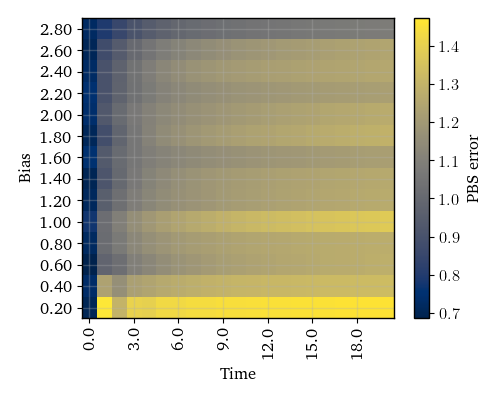
\includegraphics[width=0.6\textwidth]{Figures/bias_time_imshow.png}
	\hspace{1em}
	\caption{PBS Errors as a function of bias and time. Bias acts as a damper: when bias is higher the model take longer to over-estimate the change in opinion.}
	\label{fig:bias_slowdown}
\end{figure}

\Cref{fig:bias_slowdown} shows the relation between the bias factor and the PB
score, showing that the bias does not improve the model's predictive power. As
one might expect a bias is ``slowing down'' the model. Because of this the
model is slower to diverge away from the true opinions.

We suspect ego improves predictive accuracy for two reasons. First, by
assigning individual-specific biases, the model better reflects heterogeneous
deliberative behavior. Second, increased self-bias slows down convergence,
preventing the model from over-correcting.

\subsection{Convergence}

From \Cref{theory}, we have seen that in the limit some matrices are
convergent, while some are not, in particular if the matrix is aperiodic, it
is convergent. As we model the deliberation group as having fully connected
matrices, with self-loops, the matrices are aperiodic, and thus convergent. We look at the
distance between the estimated support matrix, and the true support matrix, to
get a sense of the rate of convergence. The distance is defined as the
$\ell_1$ norm.

\begin{figure}[ht]
	\begin{center}
		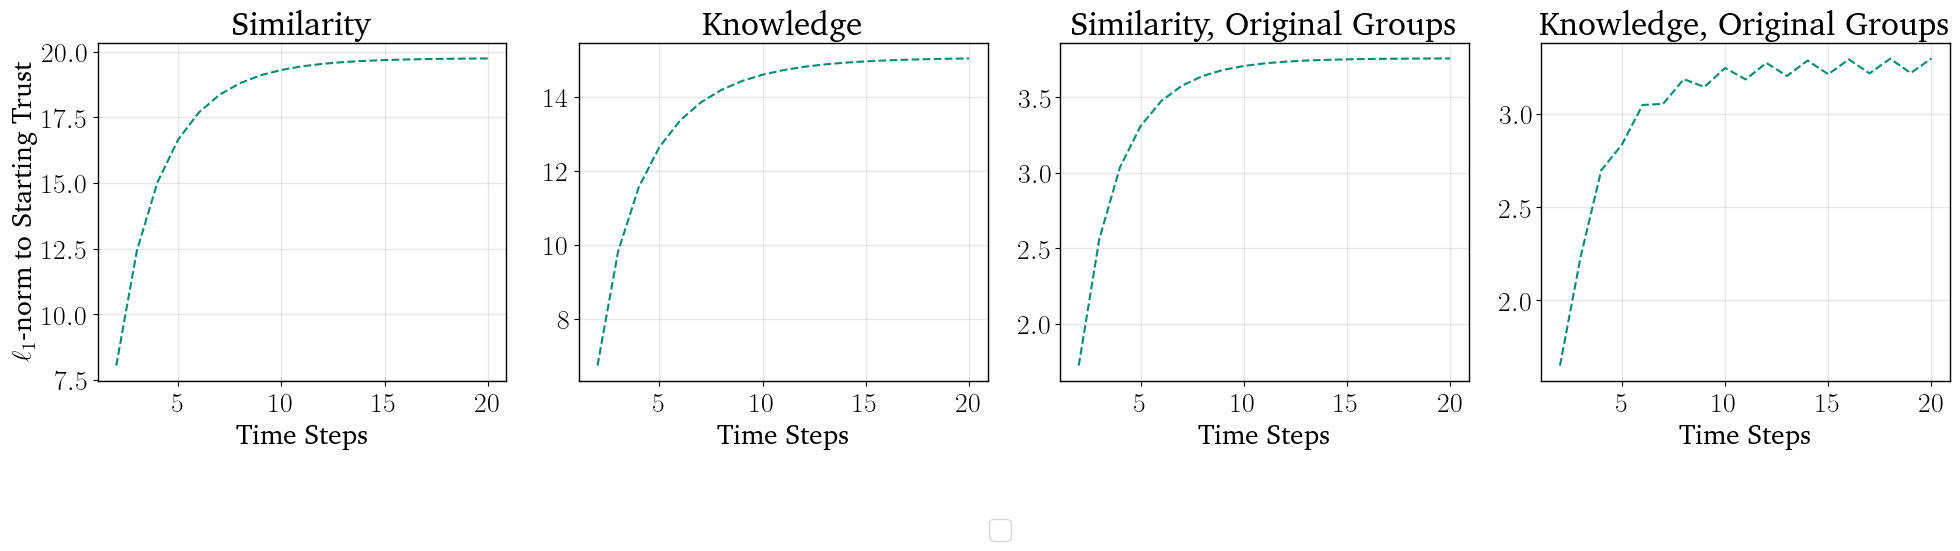
\includegraphics[width=0.95\textwidth]{Figures/convergence_groups.png}
	\end{center}
	\caption{Convergence of trust matrices, as measured by the $\ell_1$-norm between the trust matrix at the start and  trust matrix at the current time step.}\label{fig:convergence_big}
\end{figure}

In \Cref{fig:convergence_big}, we see that all configurations converge at a
similar rate, slowing down the rate of change around t = 15. Since using the
original groups leads to generally smaller groups, the absolute difference in
the matrices is smaller. When using knowledge-based trust there is a lower rate
of convergence




\section{Sensitivity Analysis} We perform sensitivity analysis on the predicted
PBS of the model. We do not use the original groups, as this allows us to vary
the number of voters. \Cref{fig:sensitivty_pbs} shows the sensitivity indices.
As for direct effects, as shown in the first order indices, the \textit{number
	of voters} is clearly the biggest factor in the variance of the model. As
expected the \textit{bias} does not directly contribute to the variance in the
model. \textit{Knowledge} informed trust and\textit{ knowledge} informed bias
(self knowledge) both are significantly impacting the variance of the model.
The second order indices show \textit{number of voters} interacts with
\textit{knowledge}, \textit{self knowledge}, and\textit{ similarity},
contributing a large portion of their explained total variance induced by the
\textit{number of voters}. There is also an interaction between \textit{ego}
and \textit{similarity} and \textit{self knowledge}. As for the Total order
indices, we see that variables contribute significantly to the variance in the
model.


\begin{figure}[ht]
	\begin{center}
		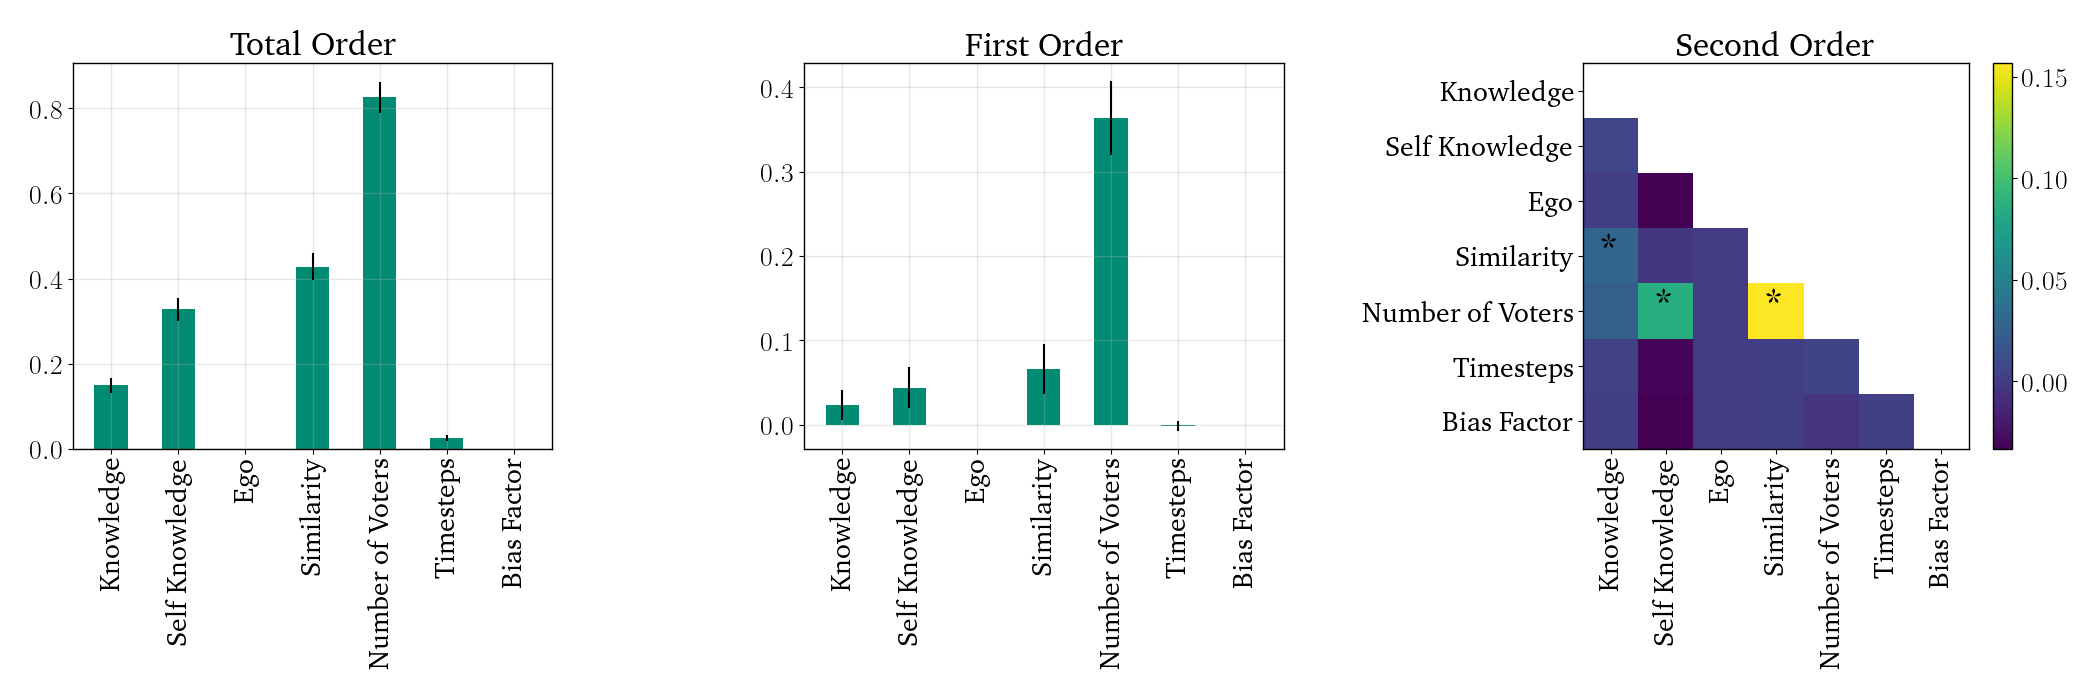
\includegraphics[width=0.95\textwidth]{Figures/senstivity_analysis.png}
	\end{center}
	\caption{First, Second and Total sensitivity indices on the PBS prediction error. The stars in the heat map for the Second order sensitivity indices indicate significant interactions. }\label{fig:sensitivty_pbs}
\end{figure}


\section{Adding Meta-Agreement}

\begin{figure}[htbp]
	\centering
	\centering
	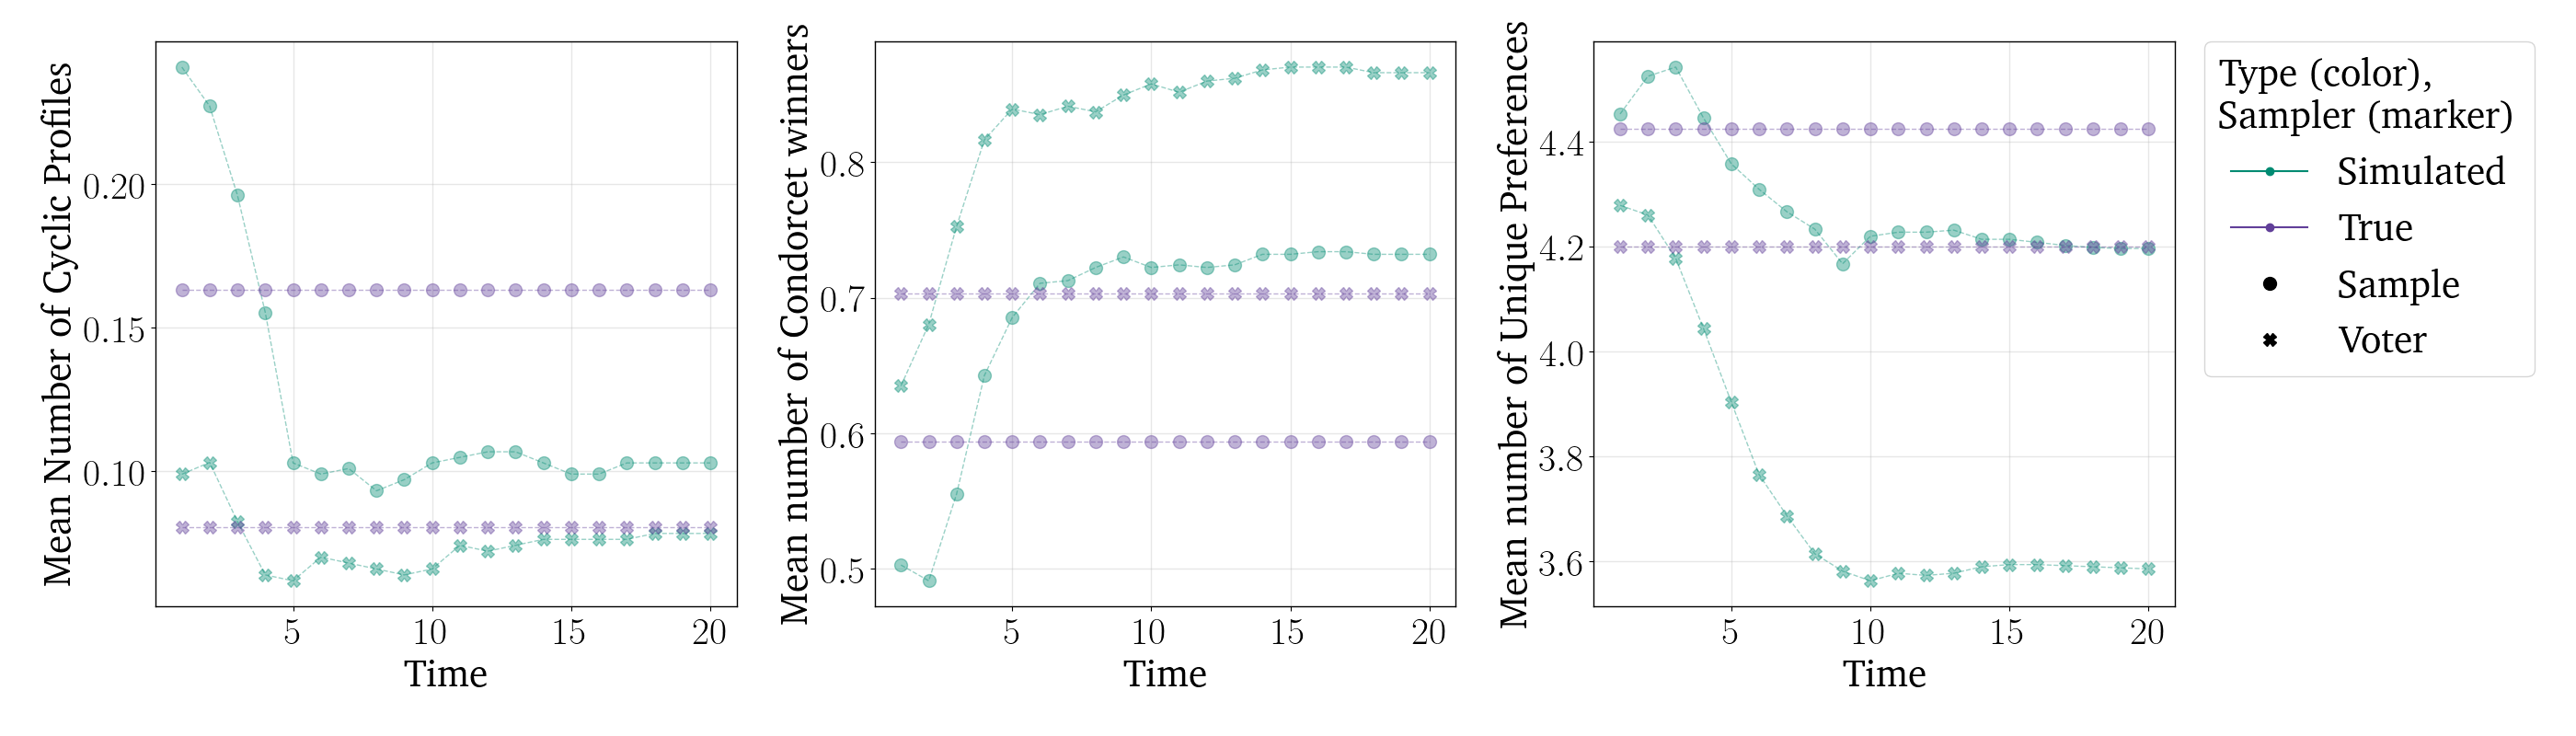
\includegraphics[width=\textwidth]{Figures/three_measures.png
	}
	\caption{The proportion of cyclic profiles remaining, 0 indicating that no cyclic profiles were present after deliberation.}
	\label{fig:degroot_cyclic}
\end{figure}

Firstly, when comparing different voter generation mechanisms, we find that generating a candidate by copying the opinion of a single voter performs best—both in minimizing the number of cyclic profiles and in maximizing the frequency with which a Condorcet winner exists. Though this result may seem unintuitive, we suspect the reason is that pre-deliberation opinions were relatively polarized. As a consequence, constructing candidates as averages of 10 voters tends to produce alternatives that are too similar, making it difficult for any one to stand out.

In contrast, a single voter's opinion is more likely to fall near a large cluster of voters, making that candidate closer—on average—to the majority. In such cases, that candidate is more likely to become a Condorcet winner. Put simply, averaged candidates tend to represent moderate positions, leading to greater voter indifference between them. In these situations, small errors in perceived support can have disproportionately large effects. Meanwhile, candidates based on a single voter's opinion—especially in a polarized society—are more likely to be distinct and strongly preferred.

Looking at the evaluation metrics used in the model, we observe a pattern similar to that found in the substantive agreement analysis. The simulation initially starts far from the true scores, gradually moves toward them, overshoots, and finally begins to converge.

\begin{figure}[htbp]
	\centering
	\vspace{-9pt}
	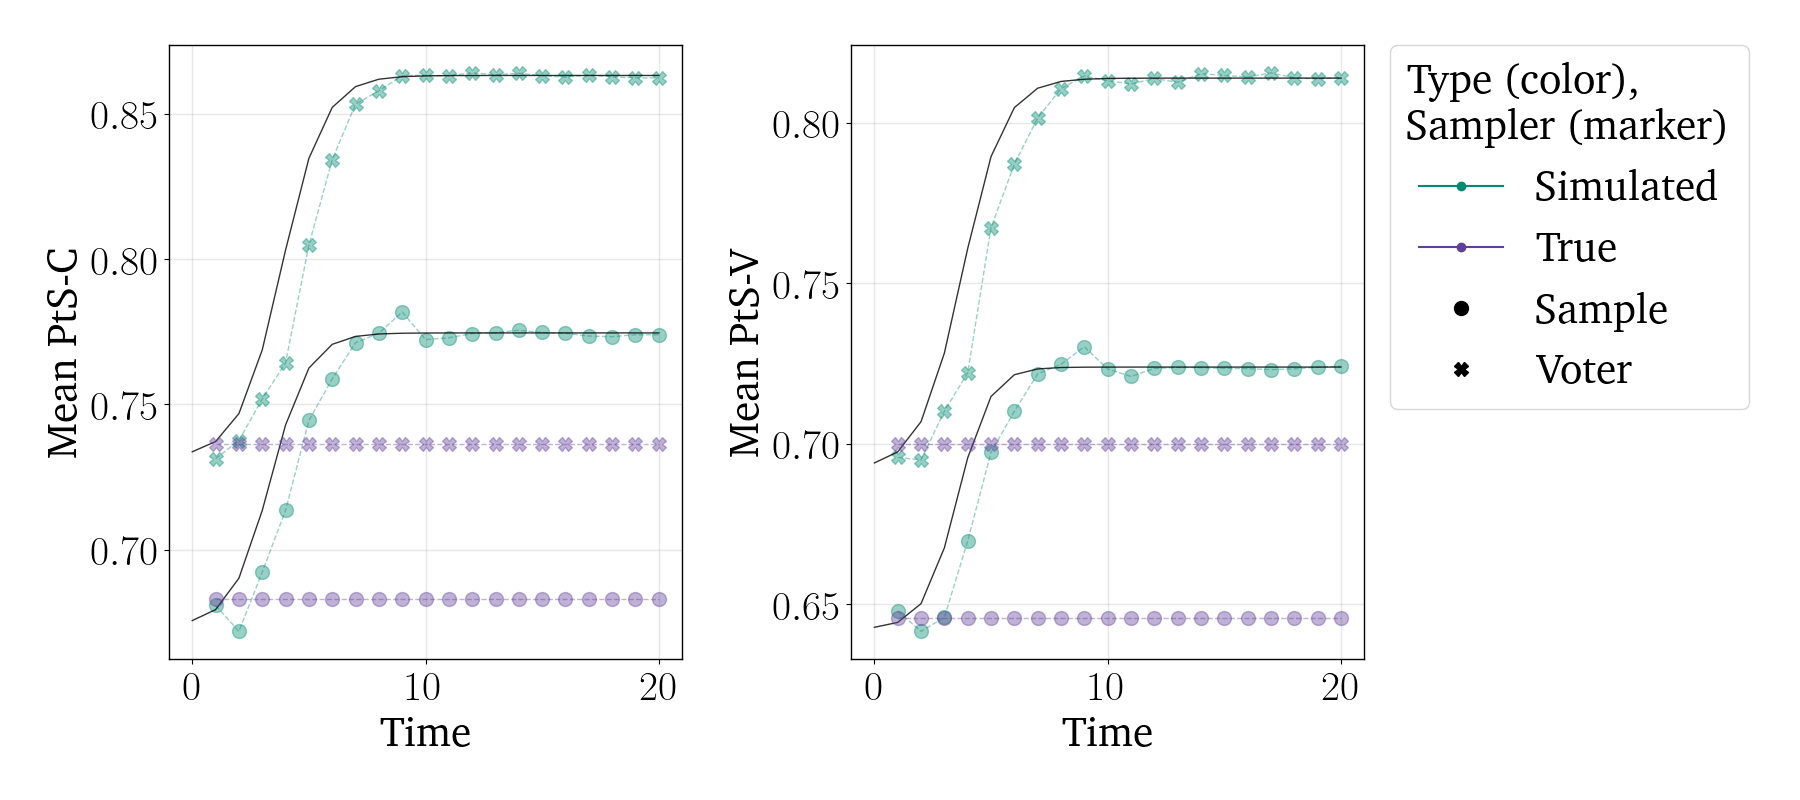
\includegraphics[width=\textwidth]{Figures/pst_measures.png}
	\caption{Proximity to single-peakedness after deliberation via candidate deletion (left) and voter deletion (right). The black line is a fitted sigmoid curve.}
	\label{fig:degroot_single_peaked}
\end{figure}

\Cref{fig:degroot_single_peaked} shows similar dynamics across simulation time for both notions of proximity to single-peakedness. Although candidate deletion and voter deletion represent two fundamentally different approaches to measuring this property, they yield a consistent conclusion: voters rapidly become more single-peaked early in the simulation, after which the rate of change slows and eventually plateaus. This behavior is well captured by a sigmoid curve, where the diminishing rate of change corresponds to the trust matrix stabilizing at its convergent state.
